% In the previous sections, we described ROMC from the user's
% point of view; the demonstration focused on performing the inference
% with the ready-to-use tools. Apart from this use-case, a practitioner
% can also use ROMC as a meta-algorithm, adding custom algorithms as
% part of the method. Our implementation allows such intervention. In
% the rest of the chapter, we will initially present the main internal
% classes, and then we will exhibit how to add custom methods.

% \subsubsection{Entities presentation}

% In figure \ref{fig:example_training} we provide an overview of the
% classes used in the algorithm. The class \code{ROMC} can be
% thought of as the interface between the user and the method. The rest of
% the classes are responsible for the back-end functionality. The reader needs to remember the sequence of the events for
% performing the inference, as demonstrated in figure
% \ref{fig:romc_overview}.

% The class \code{ROMC} is the main class of the method; it is
% initialised when the user calls the method for the first time and its
% state is updated throughout the inference. The initialisation of the
% \code{ROMC} object sets the attributes \code{model},
% \code{model_prior}, \code{bounds} and \code{inference_state} to
% the appropriate values; the rest of the attributes are set to
% \code{None}.\footnote{in all cases, we use the value None for
%   indicating that an attribute is not yet initialised."}.

% The \code{_sample_nuisance()} routine samples $n_1$ integers from
% the discrete integer distribution. The \code{_define_objectives()}
% routine initialises $n_1$ \code{OptimisationProblem} objects,
% appends them to a \code{List} and stores this \code{List} as the
% \code{romc.optim_problems} attribute. The
% \code{_define_objectives()} function, initialises only the
% attributes \code{objective} and \code{bounds} of the
% \code{OptimisationProblem}; the rest are set to \code{None}. The
% attribute \code{objective}, which is a \code{Callable}, is
% created by setting the seed of the \code{model.generate()} to a
% specific integer, turning the random generator to a deterministic.

% Afterwards, depending on the boolean argument
% \code{use_bo=True/False}, the function \linebreak \code{_solve_gradients}
% or \code{_solve_bo} is called. Both of them follow the same
% sequence of steps; for each optimisation problem they (a) solve it,
% (b) create a \code{RomcOptimisationResult} object with the solution
% and (c) store it as the \code{OptimisationProblem.result}
% attribute. Although they both apply the same sequence of steps, each
% method uses a different optimisation scheme;
% \code{_solve_gradients} uses the \code{minimize} class of the
% \code{scipy.optimize} library \cite{2020SciPy-NMeth}, whereas
% \code{_solve_bo} uses the \code{BoDeterministic} class.
% \code{BoDeterministic} is a class we implemented for performing
% Bayesian Optimisation and fitting a Gaussian Process surrogate model
% to the objective function. It relies on the Gpy framework
% \cite{gpy2014} for fitting the Gaussian Process. The only
% difference between \code{_solve_gradients} and \code{_solve_bo},
% as effect in the state of the \code{OptimisationProblem} class, is
% the initialisation of the attribute 
% \code{OptimisationProblem.surrogate}, which is done only by
% \code{_solve_bo}. The attribute is set to a \code{Callable} that
% wraps the \code{GPyRegression.predict_mean} function. If
% \code{_solve_gradients} is called, the attribute remains
% \code{None}.

% At this level, all optimisation problems have been solved. The method
% \code{_filter_solutions} is used for discarding the optimisation
% results that are over the threshold. Afterwards, \code{_build_boxes}
% estimates the bounding boxes around the accepted objective
% functions. For each accepted objective function, a
% \code{RegionConstructor} object is initialised in order to
% construct the region. In the current implementation, for each
% objective function, we construct a single bounding box, but this may
% change in a future approach; for being able to support multiple
% bounding boxes per objective function, we decided to return a
% \code{List} of \code{NDimBoundingBox} objects\footnote{Each
%   \code{NDimBoundingBox} object represents a region.}. The
% \code{List} is stored as the \code{OptimisationProblem.regions}
% attribute.

% By now, we have estimated the bounding boxes around the optimal
% points. The last step, before defining the posterior, is the fitting
% local surrogate models. This step is optional and is performed only
% if the argument \code{fit_models} is set to \code{True}. The
% routine \code{_fit_models}, fits a quadratic model on the area
% around the optimal point for each objective function. For achieving
% so, it asks for samples from the \code{NDimBoundingBox} object and
% evaluates them using the \code{OptimisationProblem.objective}
% function. Afterwards, based on these points, it fits a quadratic model
% using the \code{linear_model.LinearRegression} and
% \code{preprocessing.PolynomialFeatures} functions of the
% \code{scikit-learn} package \cite{scikit-learn}. The trained
% model is stored as the attribute
% \code{OptimisationProblem.local_surrogate}.


% Finally, the \code{_define_posterior} method is used for creating
% the \code{RomcPosterior} object and storing it as the
% \code{ROMC.posterior} attribute. The method collects (a) all the
% bounding boxes created so far (accessing the
% \code{OptimisationProblem.regions} attributes and (b) all the objective functions. As the objective function it collects either \code{OptimisationProblem.local_surrogate} or \linebreak \code{OptimisationProblem.surrogate} or \code{OptimisationProblem.objective}, depending on which one is available based on the previous steps.

% The description above summarises the sequence of steps needed for the
% training part of the method. The conclusion is that a \code{ROMC}
% object is initialised when the user calls the method. Throughout the
% inference process, the \code{ROMC} object is always as a specific state,
% which gets updated whenever an algorithmic step is executed. The rest
% of the classes provide objects which are stored as attributes of
% \code{ROMC}.

% % \begin{figure}[!h]
% %     \begin{center}
% %       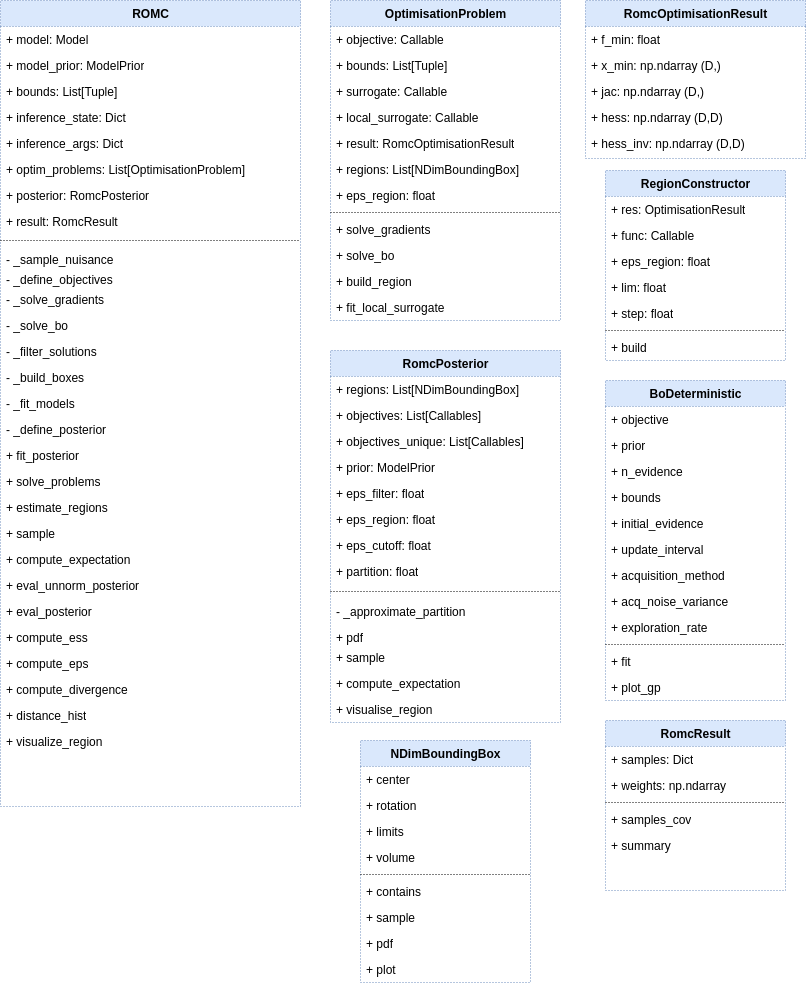
\includegraphics[width=\textwidth]{./latex_files/graphs/RomcEntityDiagram.png}
% %     \end{center}
% %   \caption[Overview of the entities (classes) of the ROMC implementation.]{Overview of the entities (classes) used at the deployment of the ROMC inference method, at the \code{ELFI} package.}
% %   \label{fig:example_training}
% % \end{figure}


% \subsubsection{Extensibility of the ROMC method}

% In this section, we will explain how a practitioner may replace some
% parts of the ROMC method with their custom algorithms. We can locate
% at least four such points; (a) the gradient-based solver, (b) the
% Bayesian Optimisation solver, (c) the bounding box region construction
% and (d) the fitting of the local surrogate models. Each of the
% tasks above may be approached with completely different
% algorithms than the ones we propose, without the rest of the method to
% change.

% The four replacable parts described above, are solved using the four
% methods of the \linebreak \code{OptimisatioProblem} class;
% \code{solve_gradients(**kwargs)}, \code{solve_bo(**kwargs)}, \linebreak
% \code{build_region(**kwargs)},
% \code{fit_local_surrogate(**kwargs)}. Therefore, the practitioner
% should not alter at all the basic \code{ROMC} class. Instead, they
% should deploy a custom optimisation problem class which inherits the
% basic \code{OptimisatioProblem} class and overwrites the above four
% functiones with custom ones. The only rule that should be followed
% carefully, is that the cutom methods must have the same effect on the
% attributes of the \code{ROMC} class, i.e. update them with the
% appropriate objects as presented in table \ref{tab:extensibility}. For
% example, a function that replaces \code{solve_gradients()} must
% have the effect of storing a \code{RomcOptimisationResult} object
% to the \code{OptimisationObject} attribute.

% \begin{center} \label{tab:extensibility} \captionof{table}[Demonstration of the appropriate effect of each replaceable routine]{Table
%     explaining the appropriate effect of each replaceable routine,
%     i.e. which object they should attach to the appropriate
%     attribute. The functions of the first column (\code{ROMC}
%     class) call the corresponding functions of the second column
%     (\code{OptimisationProblem} class). The functions of the second
%     column should execute their main functionality and update the
%     appropriate attribute with a certain object, as described in the
%     third column. }


% \begin{tabular}{ c|c }
% \hline
% \code{OptimisationProblem} & \code{Effect} \\
% \hline \hline
% \code{solve_gradients()} & \code{result <- RomcOptimisationResult} \\
% \hline
% \multirow{2}{*}\text{\code{solve_bo()}} & \text{\code{result <- RomcOptimisationResult}} \\
%  & \text{\code{surrogate <- Callable}} \\
% \hline
% \code{build_region()} & \code{regions <- List[NDimBoundingBox]}\\
% \hline
% \code{fit_local_surrogate()} & \code{local_surrogate <- Callable}\\
% \hline
% \end{tabular}
% \end{center}

% \subsubsection*{Example: use a Neural Network as a local surrogate model}

% Let's say we have observed that the local area around $\theta_i^*$ is
% too complex to be represented by a simple quadratic model\footnote{as
%   in the current implementation}. Hence, the user selects a neural
% network as a good alternative. In the following snippet, we
% demonstrate how they could implement this enhancement without much
% effort; (a) they have to develop the neural network using the package
% of their choice (b) they must create a custom optimisation class which
% inherits the basic \code{OptimisationClass} and (c) they have to
% overwrite the \code{fit_local_surrogate} routine, with one that
% sets the neural network's prediction function as the
% \code{local_surrogate} attribute. The argument \code{**kwargs}
% may be used for passing all the important arguments, e.g.\ training
% epochs, gradient step etc. If, for example, they would like to set the
% size of the training set dynamically, we may replace \code{x =
%   self.regions[0].sample(30)} with \code{x =
%   self.regions[0].sample(kwargs["nof_examples"])}. Finally, they must
% pass the custom optimisation class, when calling the \code{ROMC}
% method.

% \begin{Code}
% ------------------------------ python snippet ------------------------------  
%   class NeuralNetwork:
%       def __init__(self, **kwargs):
%           # set the input arguments

%       def train(x, y):
%           # training code

%       def predict(x):
%           # prediction code

%   # Inherit the base optimisation class
%   class customOptim(elfi.methods.parameter_inference.OptimisationProblem):
%       def __init__(self, **kwargs):
%           super(customOptim, self).__init__(**kwargs)

%       # overwrite the function you want to replace
%       def fit_local_surrogate(**kwargs):
%           # init and train the NN
%           x = self.regions[0].sample(30) # 30 training points
%           y = [np.array([self.objective(ii) for ii in x])]
%           nn = NeuralNet()
%           nn.train(x,y)

%           # set the appropriate attribute
%           self.local_surrogate = nn.predict

%           # update the state
%           self.state["local_surrogate"] = True

%   # pass the custom inference method as argument
%   romc = elfi.ROMC(dist, bounds, custom_optim_class=customOptim)
% ----------------------------------------------------------------------------
% \end{Code}
